\documentclass{article}
\usepackage[utf8]{inputenc}
\usepackage{amsmath}
\usepackage{float}
\usepackage{fullpage}
\usepackage{parskip}
\usepackage{graphicx}
\usepackage{subcaption}

\title{Ph20 Assignment 3 (Part 2)}
\author{Ung Shu Fay}

\begin{document}
\maketitle

\section{Phase Space Trajectories}
    \begin{figure}[h!]
        \centering
        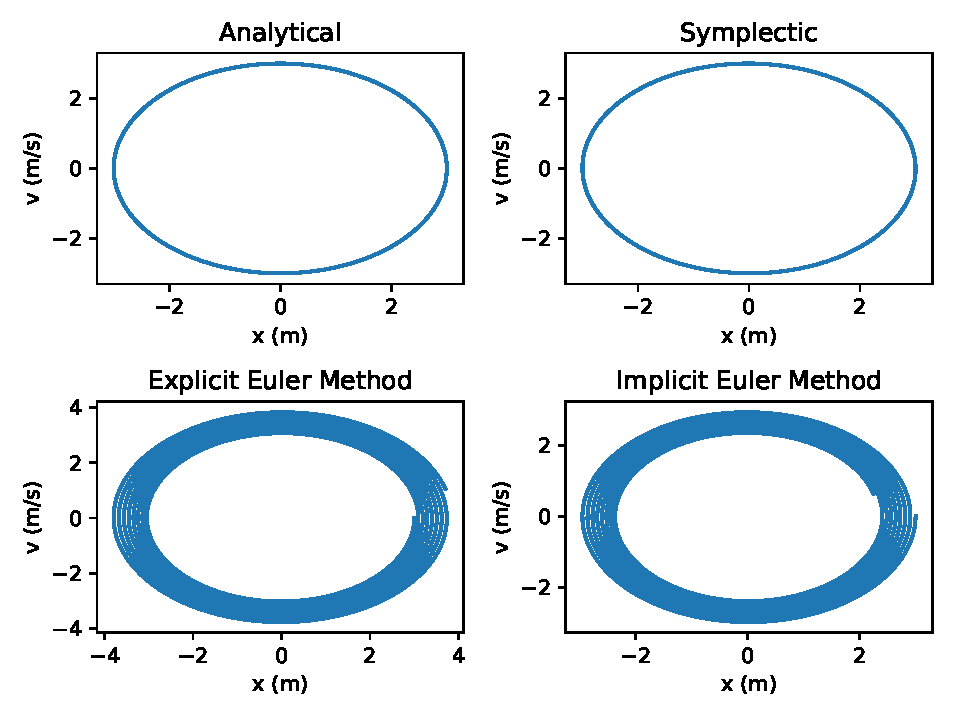
\includegraphics[scale=0.8]{phase_space.pdf}
        \caption
        {
            Phase space trajectories of solutions for the spring given by the analytical, symplectic, explicit and implicit Euler's method. The analytical and symplectic solutions trace out a circle in phase space while the Euler's methods do not trace out closed curves. The parameters were: $x_0 = 3, v_0 = 3, h = 0.01, N = 5000$.
        }
        \label{phase}
    \end{figure}
    
    The circular trajectory produced by the symplectic Euler method shows that its solution replicates the behaviour of the analytical solution in phase space, unlike the explicit and implicit Euler methods. 
    
\break
\section{Energy}
    \begin{figure}[h!]
        \centering
        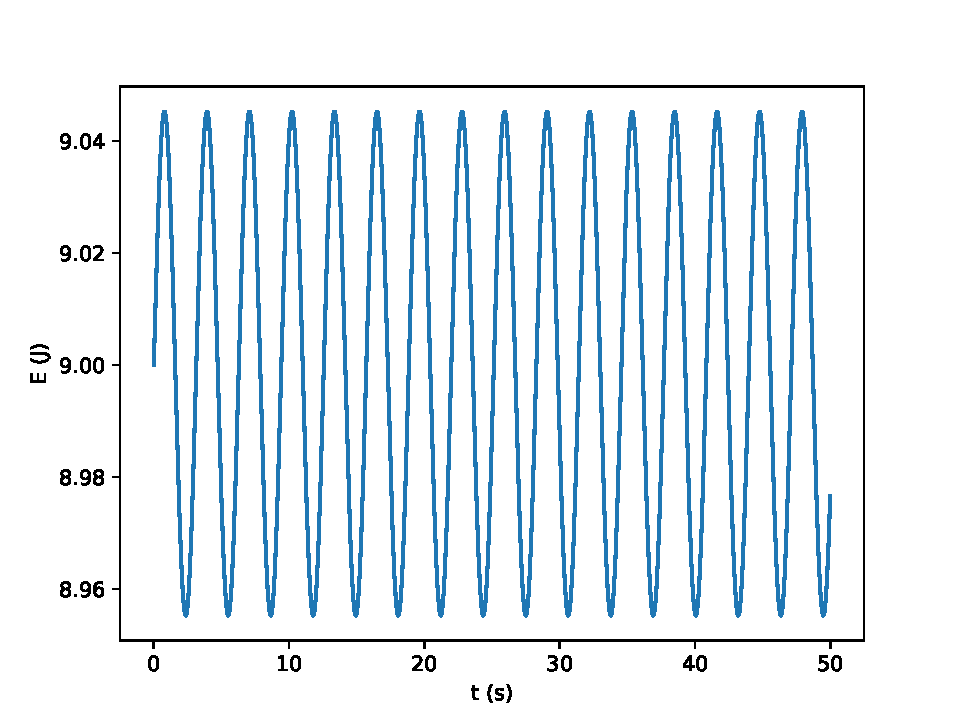
\includegraphics[scale=0.6]{energy.pdf}
        \caption
        {
            Evolution of the total energy obtained with the symplectic Euler method. The total energy as a function of time is sinusoidal. The average total energy $E= 9 \ \mathrm{J}$ is constant and produces the circle $x^2 + v^2 = E$ traced out in phase space. The plot was generated with $h = 0.01$.
        }
        \label{energy}
    \end{figure}

\section{Global Error}
    \begin{figure}[h!]
        \centering
        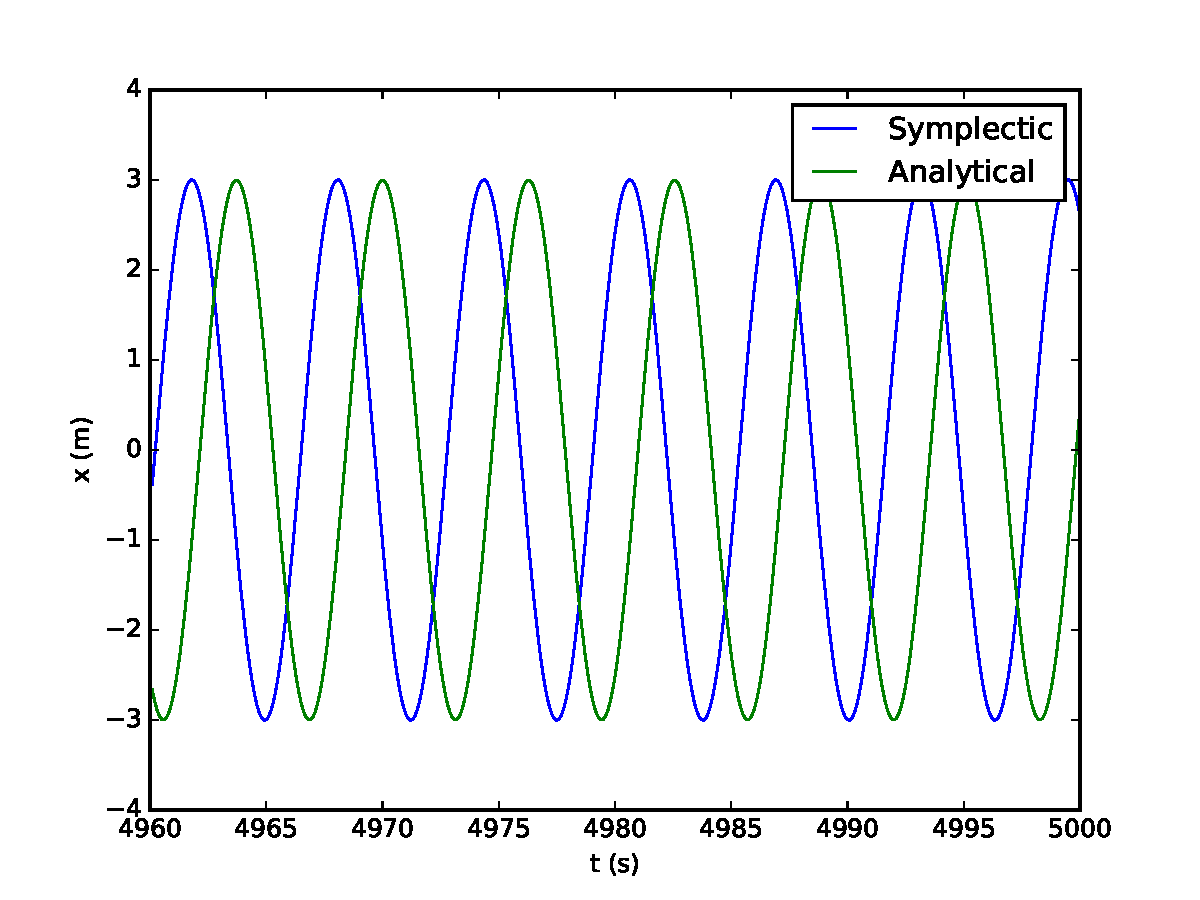
\includegraphics[scale=0.6]{error.pdf}
        \caption
        {
            Global error in phase produced by the symplectic Euler method. The plot was produced for the last 6 oscillations of 750 oscillations with $h = 0.1$ and $N = 50 \ 000$.
        }
        \label{fig:my_label}
    \end{figure}
\end{document}
